\chapter{JVM und Bytecode}
\label{cha:jvm}

Die Java Virtual Machine (JVM) ist eine von James Gosling für Sun konzipierte und in Folge von Oracle weiterentwickelte Stack-basierte virtuelle Maschine. Die JVM ermöglicht die Ausführung von Bytecode unter Linux, MacOS und Windows. Zu Beginn für die plattformunabhängige Ausführung von Java-Code entwickelt, existieren eine Vielzahl an Programmiersprachen für die JVM. Dazu gehören neben Java unter anderem Kotlin/JVM, Scala und Clojure.
Als Grundlage für dieses Kapitel dient \textcite{lindholm2016java}.

\section{HotSpot}

Neben der Übersetzung von Bytecode auf Maschinencode beinhaltet die JVM auch den \textit{Just-in-Time (JIT)} Compiler \textit{HotSpot}. Sobald die Anzahl der Aufrufe einer bestimmten Methode den Schwellwert überschreitet, übersetzt \textit{HotSpot} diese Methode in Maschinencode und ersetzt den originalen Bytecode für die restliche Ausführung des Programmes. Startet man das Programm neu, beginnt dieser Prozess von vorne. Dieser Prozess hat das Ziel, häufig verwendete Methoden zu optimieren, um dadurch die Laufzeit-Performanz zu erhöhen. Der Name stammt vom Gedanken, dass \textit{HotSpot} heiße Regionen (engl. \textit{hotspots}), also oft aufgerufene Methoden optimieren soll.

\textit{HotSpot} bietet zwei Stufen des \textit{JIT Compilers} an: Client (C1) und Server (C2) \parencite{jvmhotspot}. Der Client Compiler ist auf eine schnelle Startzeit optimiert und versucht das Programm so schnell wie möglich zu optimieren. Der Server Compiler hingegen ist auf eine hohe Leistung optimiert, weshalb das Optimierungsverfahren länger dauert, aber dafür eine höhere Programm-Performanz als Folge hat. Um nun die Vorteile von beiden Stufen ausnutzen zu können, tritt der C1 Compiler früher als der C2 Compiler in Kraft und erst sobald ein höherer Schwellwert erreicht ist, kommt es zur Optimierung durch den C2 Compiler. Die JIT-Optimierung ist in fünf Stufen aufgeteilt:
\begin{itemize}
    \item \textbf{Stufe 0}: Die JVM nimmt keine Optimierungen vor, erhebt aber Statistiken für die Optimierung in den weiteren Stufen.
    \item \textbf{Stufe 1} (C1): Die JVM kompiliert triviale Methoden, erhebt in dieser Stufe aber keine Statistiken.
    \item \textbf{Stufe 2} (C1): Die JVM verwendet diese Stufe, um sobald wie möglich die Performanz zu erhöhen und wenn die Schlange für die C2 Optimierung voll ist. Aus diesem Grund liegt der Methodenaufruf-Schwellwert dieser Stufe bei 0. Im weiteren Verlauf verwendet die JVM die dritte Stufe, um das Ergebnis dieser Stufe noch weiter zu optimieren.
    \item \textbf{Stufe 3} (C1): Dies ist die Standardstufe, welche am häufigsten in Verwendung ist. \textit{HotSpot} optimiert Methoden anhand gesammelter Statistiken, ignoriert jedoch triviale Methoden. Der Schwellwert dieser Stufe liegt bei 2000 Methodenaufrufen.
    \item \textbf{Stufe 4} (C2): Dies ist die einzige Stufe, bei der der C2 Compiler zum Einsatz kommt. Die Optimierung hierbei ist aufwändiger, liefert jedoch den am höchsten optimierten Code als Ergebnis. Der Schwellwert, um diese Stufe zu erreichen, liegt mit 15 000 Methodenaufrufe am höchsten.
\end{itemize}

Entscheidet sich die Entwickler:in gegen Verwendung der gestuften Kompilierung, liegt der Optimierungs-Schwellwert bei 10 000 Methodenaufrufen. Mit dem Parameter \texttt{-XX:-TieredCompilation} besteht die Möglichkeit, gestufte Kompilierung zu deaktivieren.

\section{Classloader}

Die Aufgabe des \textit{Classloaders} ist es, Klassen bei Bedarf dynamisch während der Laufzeit nachzuladen und zu verknüpfen. \textit{Classloader} sind in einer Baumstruktur aufgebaut, an deren Wurzel der \textit{Bootstrap-Classloader} steht. Dieser \textit{Bootstrap-Classloader} lädt interne Klassen der Java Plattform und ist Ausgangsbasis für alle weiteren \textit{Classloader}. Neben dem \textit{Bootstrap-Classloader} gibt es standardmäßig noch den \textit{Erweiterungs}- und \textit{System-Classloader}. Der \textit{Erweiterungs-Classloader} lädt Erweiterungen der primären Java Klassen. Der \textit{System-Classloader} hat als Aufgabe, Klassen des ausgeführten Java-Programms, der \textit{Classpath}-Umgebungsvariable und des \textit{Classpath}-Kommandozeilen\break-parameters nachzuladen.

\section{Laufzeitdatenbereiche}

Der Laufzeitdatenbereich dient zum Speichern von Variablen, Objekten und Methoden. Ebenso umfasst es Strukturen, die Informationen über den momentanen Zustand eines Programmes enthalten. Die Architektur der JVM hinsichtlich der Laufzeitdatenbereiche ist in~\autoref{fig:jvm-architecture} zu sehen.

Die JVM unterstützt die Erzeugung einer beliebigen Anzahl an Threads. Jeder dieser Threads besitzt ein \texttt{pc} Register, welches die Adresse der momentan ausgeführten Anweisung enthält.

Sowie jeder Thread ein \texttt{pc} Register besitzt, besitzt auch jeder Thread einen \textit{Java Virtual Machine stack} (von hier an Stack genannt). Dieser Stack stellt einen Stapel von \textit{Frames} dar. Frames sind Elemente variabler Größe und speichern lokale Variablen und partielle Ergebnisse. Stacks können sowohl mit einer fixen Größe, als auch dynamisch nach Bedarf der JVM definiert sein. Übersteigt die benötigte Stack-Größe die maximal erlaubte Größe, so kommt es zu einem \texttt{StackOverflowError}.

Zusätzlich zum Stack besitzt die JVM auch noch den Heap, ein Speicherbereich, den sich im Gegensatz zu \texttt{pc} Register und Stack alle Threads teilen. Im Heap liegen alle Felder und Klassen-Instanzen. Die JVM verfügt über eine automatische Speicherbereinigung, wenn Objekte nicht mehr benötigt werden: Der sogenannte \textit{Garbage Collector}. Deshalb gibt es auch keine Mechanismen, Speicherplatz von Objekten freizugeben.

Im Methodenbereich liegen Strukturen, wie zum Beispiel der Bereich für Laufzeitkonstanten (\textit{Run\-Time Constant Pool}), Klassenvariablen, Methoden und Inhalt der Methoden. Im Bereich für Laufzeitkonstanten liegen Wertliterale und Referenzen auf Methoden und Klassen und dient als eine Art Tabelle, aus welcher das Programm Werte referenzieren kann.  Der Methodenbereich stellt einen Unterbereich des Heaps dar, muss aber im Gegensatz zum Heap nicht zwingend der automatischen Speicherbereinigung unterliegen.

Um Interoperabilität mit anderen Programmiersprachen zu gewährleisten, benötigt es den nativen Methoden Stack. Native Methoden innerhalb dieses Stacks sind unabhängig von Restriktionen der JVM, können jedoch auf deren Datenbereiche zugreifen. Kommt es zum Aufruf einer nativen Methode, so wechselt die JVM vom herkömmlichen Stack zum nativen Methoden Stack, führt diese Methode aus und liefert, wenn vorhanden, ein Ergebnis zurück.

\begin{figure}
    \caption{Architektur der JVM Laufzeitdatenbereiche}
    \centering
    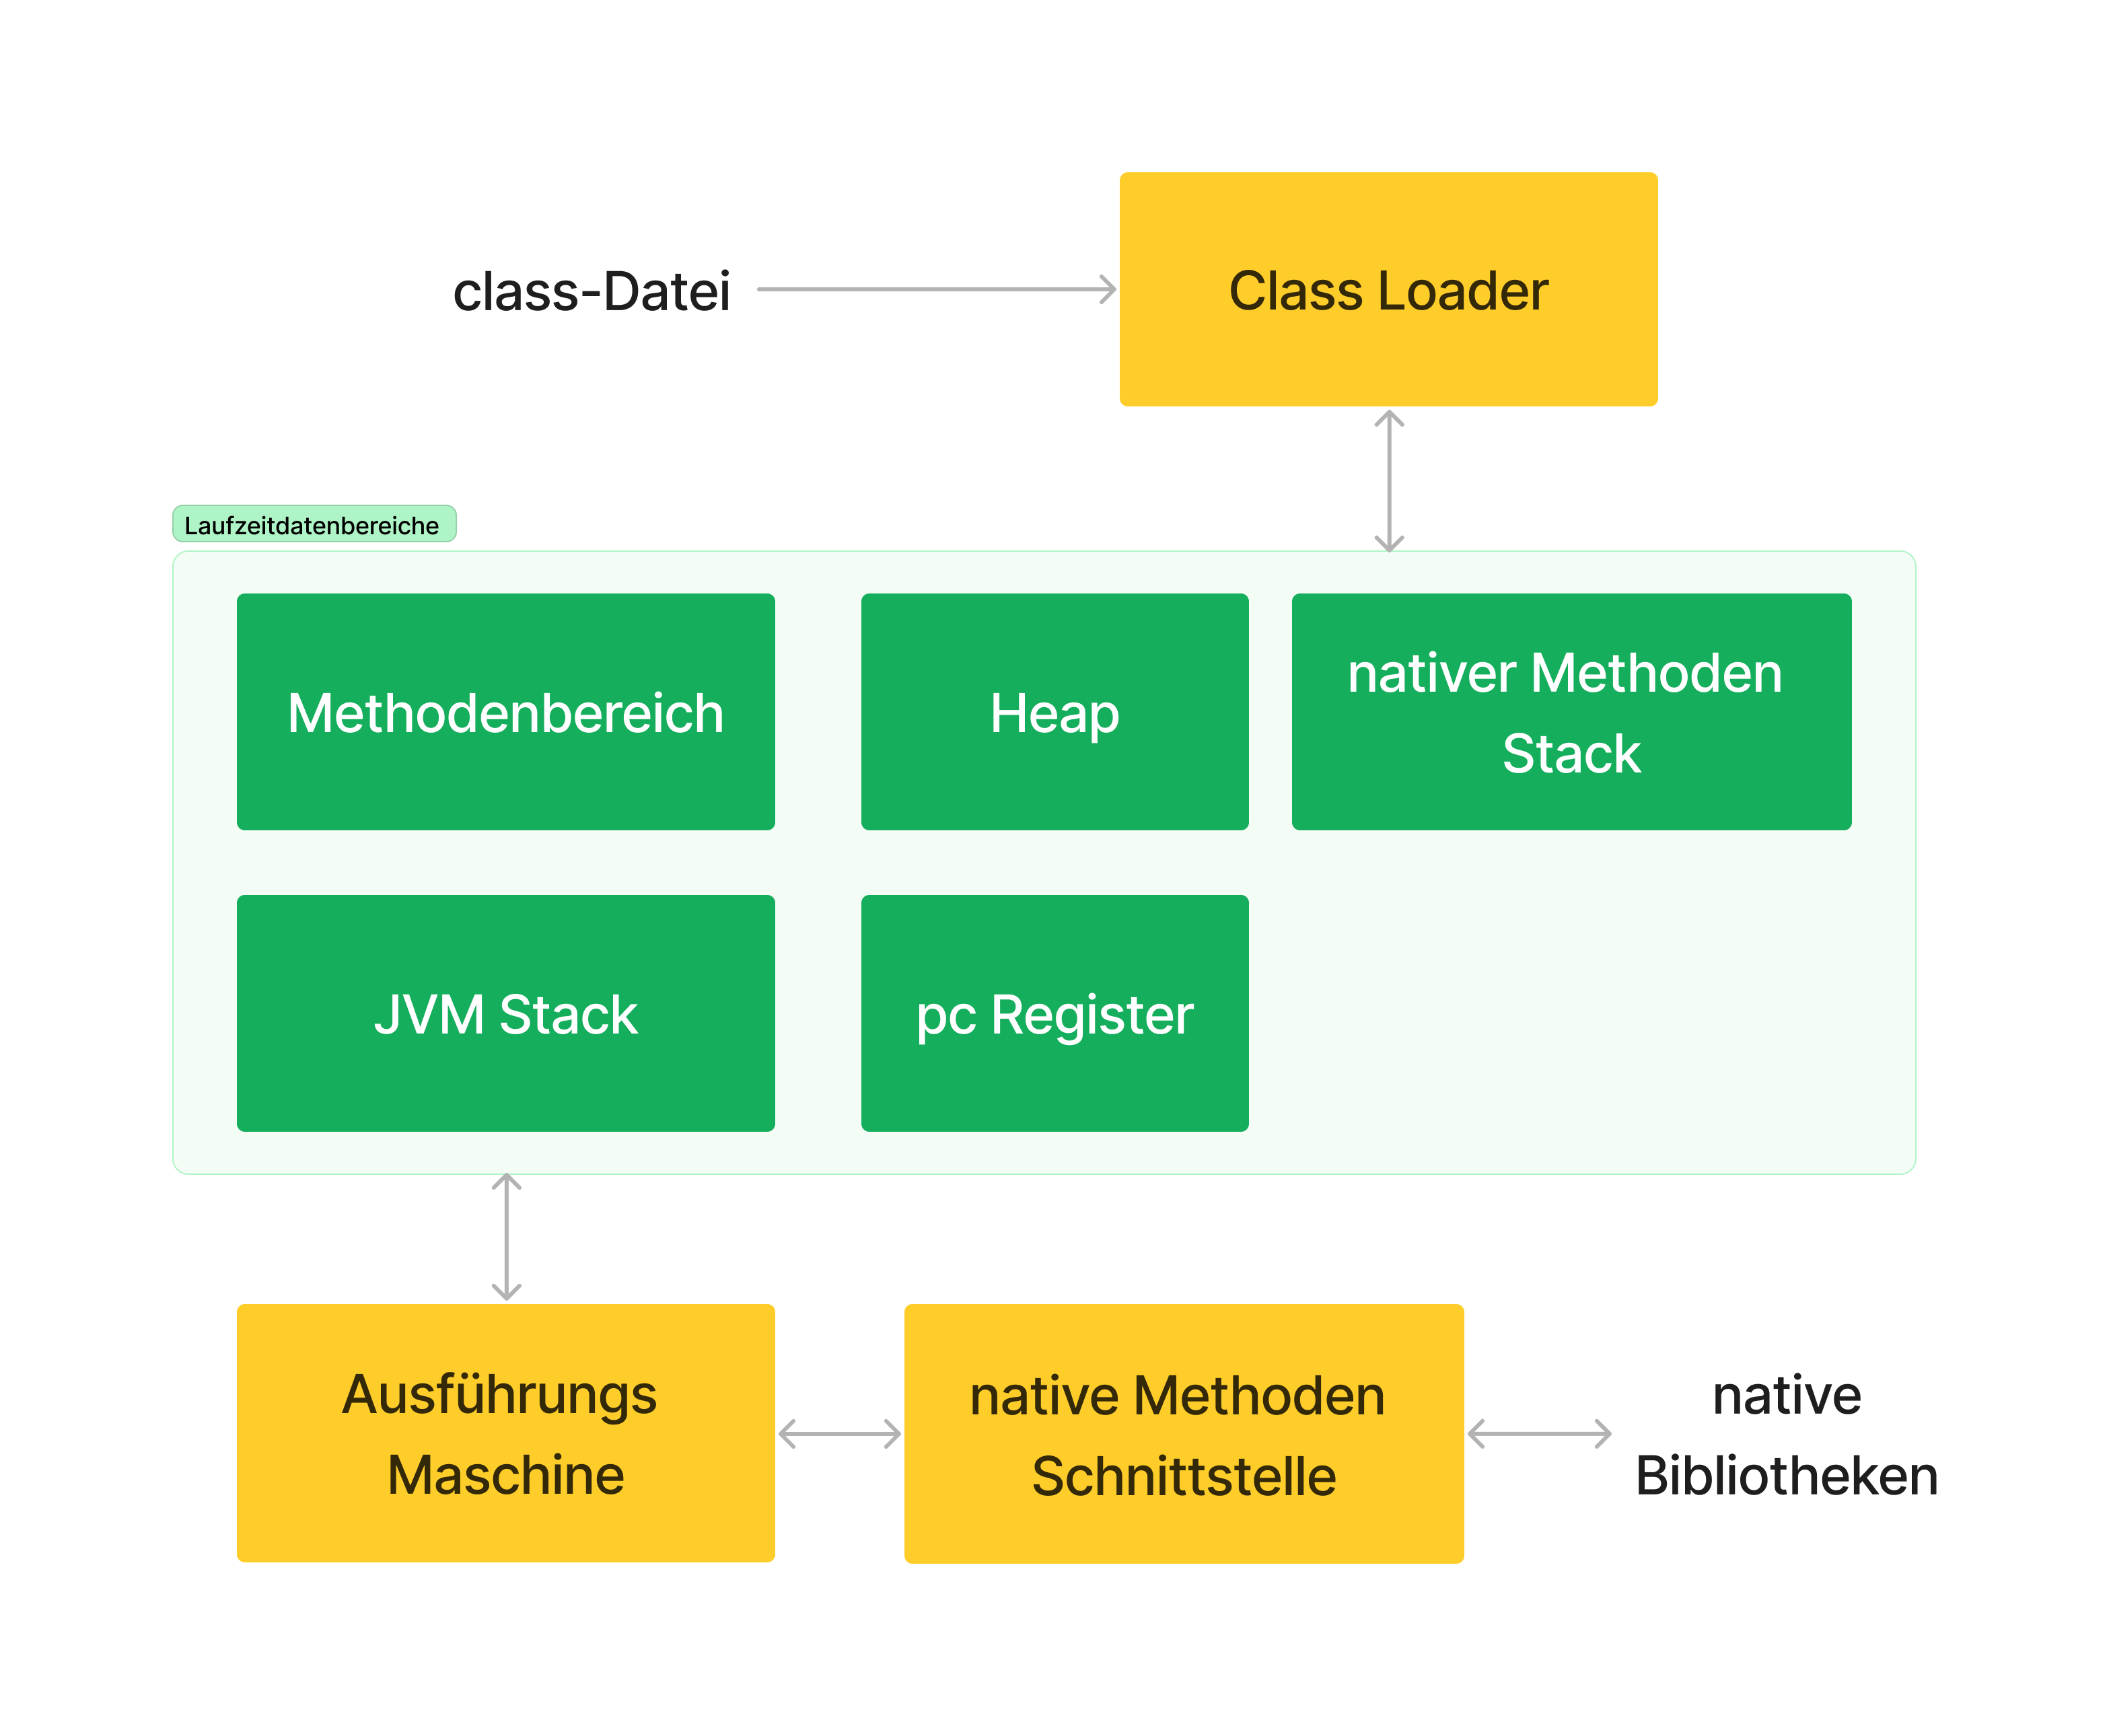
\includegraphics[width=\textwidth]{JVM.Architecture}
    \label{fig:jvm-architecture}
\end{figure}

\section{Bytecode}

Da die JVM nicht direkt den Code von JVM-basierten Programmiersprachen lesen kann, benötigt es eine Zwischensprache, den Bytecode. Dieser Bytecode entsteht bei der Übersetzung von JVM-basierten Programmiersprachen. Die class-Dateien, die bei der Übersetzung des Quelltextes erzeugt werden, enthalten als Resultat diesen Bytecode innerhalb der Methodenrümpfe.

Eine Anweisung des Bytecodes besteht aus einem Opcode, auch \textit{mnemonic} genannt, gefolgt von keinem oder mehr Operanden. Oft folgen dem Opcode keine Operanden.~\autoref{lst:jvm_bytecodeloop} zeigt die illustrative Schleife, die den Bytecode interpretiert, \cite[siehe S. 25]{lindholm2016java}.

\begin{JavaCode}[numbers=none, caption={Auszug aus der JVM Spezifikation, welche die Interpretationsschleife für Bytecode repräsentiert.}, label=lst:jvm_bytecodeloop]
do {
    atomically calculate pc and fetch opcode at pc;
    if (operands) fetch operands;
    execute the action for the opcode;
} while (there is more to do);
\end{JavaCode}

Opcodes sind für die verschiedenen Typen der JVM separat implementiert. Will die Entwickler:in zum Beispiel zwei Variablen vom Typ \texttt{int} und \texttt{double} laden, um diese später zu addieren, müssen diese im ersten Schritt mit den beiden Opcodes \texttt{iload} und \texttt{dload} geladen werden. Nach dem Laden der beiden Werte liegen diese nun am Operanden-Stack.

Einige Opcodes, \texttt{iload} unter anderem, haben zusätzliche Varianten, die einen Suffix im Format \texttt{\_<number>} enthalten. Das Verhalten dieser Opcodes unterscheidet sich nicht von den suffixlosen Varianten, sondern dient als Speicherplatzsparmaßnahme. Die Zahl am Ende des Suffixes stellt den Index im lokalen Variablenfeld dar, auf das der Opcode zugreift. Dadurch vermeidet die JVM die Notwendigkeit eines zusätzlichen Parameters für häufig verwendete Indizes und spart ein Byte Speicherplatz.  Die Anzahl an Varianten ist je nach Opcode unterschiedlich. \texttt{iload} bietet zum Beispiel \texttt{iload\_0} bis \texttt{iload\_3}. 

Da es sich dabei um zwei verschiedene Typen handelt, konvertiert man den kleineren Typ (in diesem Fall \texttt{int}) zum größeren Typ mit dem Opcode \texttt{i2d}. Vom Namen lässt sich ableiten, dass diese Anweisung die Ganzzahl zu einer Gleitkommazahl konvertiert. Wichtig hierbei ist, dass der zu konvertierende Wert oben am Operanden-Stack aufliegen muss, da die Operation \texttt{i2d} den obersten Wert des Operanden-Stack entnimmt und den konvertierten Wert anschließend zurücklegt.

Mit zwei Gleitkommawerten kann man nun anschließend \texttt{dadd} aufrufen. Diese Operation entnimmt die beiden obersten Werte dem Operanden-Stack, errechnet die Summe und legt diese anschließend wieder auf den Operanden-Stack.

All diese Operationen sind für alle weiteren Typen der JVM definiert und sind der Spezifikation zu entnehmen. Die Größe aller Opcodes ist zugunsten der Kompaktheit auf ein Byte beschränkt. Daraus ergibt sich eine maximale Anzahl von 256 Opcodes.